% Build: module load texlive/20240312-GCC-13.3.0 && latexmk -pdf rebuild_talk.tex

\documentclass[11pt,aspectratio=169]{beamer}

% ---------------------------------------------------------------------------
% Look: plain beamer, Yale colours
% ---------------------------------------------------------------------------
\usetheme{default}
\usefonttheme{professionalfonts}
\setbeamertemplate{navigation symbols}{}

\definecolor{yaleblue}{HTML}{00356B}
\definecolor{yalemid}{HTML}{286DC0}
\definecolor{yalelight}{HTML}{63AAFF}
\definecolor{yalegrey}{HTML}{4A4A4A}
\definecolor{yalelightgrey}{HTML}{DDDDDD}

\setbeamercolor{structure}{fg=yaleblue}
\setbeamercolor{normal text}{fg=black}
\setbeamercolor{frametitle}{fg=yaleblue}
\setbeamercolor{title}{fg=yaleblue}
\setbeamercolor{alerted text}{fg=yalemid}
\setbeamercolor{block title}{fg=white,bg=yaleblue}
\setbeamercolor{block body}{bg=yalelightgrey!40}

\setbeamerfont{frametitle}{series=\bfseries,size=\large}
\setbeamerfont{title}{series=\bfseries,size=\Large}

\setbeamertemplate{itemize items}[circle]
\setbeamertemplate{blocks}[rounded][shadow=false]

% A thin blue rule under each frame title
\setbeamertemplate{frametitle}{%
  \vspace*{0.6em}%
  \usebeamerfont{frametitle}\usebeamercolor[fg]{frametitle}\insertframetitle\par
  \vspace*{-0.2em}{\color{yaleblue}\rule{\textwidth}{0.6pt}}%
}

% Footer: short title on the left, slide number on the right
\setbeamertemplate{footline}{%
  \hspace*{1.2em}{\color{yalegrey}\scriptsize\insertshorttitle}%
  \hfill{\color{yalegrey}\scriptsize\insertframenumber}\hspace*{1.2em}%
  \vspace*{0.6em}%
}

% ---------------------------------------------------------------------------
% Packages
% ---------------------------------------------------------------------------
\usepackage[T1]{fontenc}
\usepackage{lmodern}
\usepackage{booktabs}
\usepackage{array}
\usepackage{graphicx}
\usepackage{amsmath}
\usepackage{tikz}
\usetikzlibrary{positioning,arrows.meta,calc}
\usepackage{pgfplots}
\pgfplotsset{compat=1.18}
\graphicspath{{figures/}}

% Diagram styles
\tikzset{
  tok/.style={draw=yaleblue, rounded corners=2pt, font=\small, inner sep=4pt,
              minimum height=0.65cm},
  blank/.style={tok, fill=yalelight!35, font=\small\bfseries},
  box/.style={draw=yaleblue, rounded corners=2pt, font=\scriptsize, align=center,
               text width=2.1cm, minimum height=1.1cm, inner sep=3pt},
  arr/.style={-{Stealth[length=5pt]}, yaleblue, thick},
  cF/.style={fill=yaleblue},
  cP/.style={fill=yalelight!60},
  cN/.style={fill=white},
}

\pgfplotsset{colormap={yalemap}{color=(white) color=(yalelight) color=(yaleblue)}}


% Distribution maps (slides on pretraining and post-training): a smooth 2D
% density from Gaussian bumps g, shaded white to Yale blue.
\pgfplotsset{sentencemap/.style={view={0}{90}, width=6.6cm, height=5.4cm,
    xmin=-3, xmax=3, ymin=-3, ymax=3, ticks=none, colormap name=yalemap,
    axis line style={yalegrey}, clip=false,
    /pgf/declare function={g(\x,\y,\a,\b,\s) = exp(-((\x-\a)^2 + (\y-\b)^2)/(2*\s^2));}}}

% Four labelled points on a distribution map, at fixed positions:
% #1 top left, #2 top right, #3 bottom right, #4 bottom left (the unrealistic one)
\newcommand{\maplabels}[4]{%
  \begin{scope}[every node/.style={font=\tiny, fill=white, fill opacity=0.8,
        text opacity=1, inner sep=1.5pt, rounded corners=1pt, align=left}]
    \fill[black] (axis cs:-1.6,1.2,5) circle (1.2pt);
    \node[anchor=south west] at (axis cs:-1.7,1.3,5) {#1};
    \fill[black] (axis cs:1.4,1.3,5) circle (1.2pt);
    \node[anchor=north, align=center] at (axis cs:1.4,1.2,5) {#2};
    \fill[black] (axis cs:1.5,-1.5,5) circle (1.2pt);
    \node[anchor=north, align=center] at (axis cs:1.5,-1.6,5) {#3};
    \fill[black] (axis cs:-2.2,-2.4,5) circle (1.2pt);
    \node[anchor=south west] at (axis cs:-2.2,-2.3,5) {#4};
  \end{scope}}

\newcommand{\recordlabels}{\maplabels{married, 38,\\ two children}{age 81, Social\\ Security \$31k}{age 70, \$400k saved,\\ \$2k interest (0.5\%)}{age 9, wages \$300k}}

% Training slide. Cells sit at column #1, row #2 of a picture with x=1.5cm, y=0.85cm.
\tikzset{
  cell/.style={tok, minimum width=1.38cm, minimum height=0.7cm, font=\scriptsize},
  hid/.style={blank, minimum width=1.38cm, minimum height=0.7cm, font=\scriptsize\bfseries},
  absent/.style={cell, draw=yalelightgrey, fill=yalelightgrey!50, text=yalegrey},
}
\newcommand{\cellv}[3]{\node[cell] at (#1,-#2) {#3};}          % a visible value
\newcommand{\cellh}[2]{\node[hid] at (#1,-#2) {?};}            % a hidden cell
\newcommand{\cella}[2]{\node[absent] at (#1,-#2) {--};}        % not in this source
% A guessed distribution: #3 the bar heights (tallest = 1), #4 the true bar
% (0 = truth not shown yet), #5 the true value
\newcommand{\cellg}[5]{%
  \node[hid] at (#1,-#2) {};
  \foreach \hgt [count=\k] in {#3} {
    \ifnum\k=#4 \def\barcol{yaleblue}\else\def\barcol{yalemid!40}\fi
    \fill[\barcol] ($(#1,-#2)+(-0.75cm+\k*0.15cm,-0.27cm)$) rectangle ++(0.1cm,\hgt*0.5cm);
  }
  \ifnum#4>0 \node[font=\tiny, text=yaleblue] at ($(#1,-#2)+(0.4cm,0)$) {#5};\fi
}
% The network strip under the table: idle, guess (arrows on), or update (weights lit)
\newcommand{\trainnet}[1]{%
  \begin{scope}[shift={(5,-5.5)}, x=1cm, y=1cm]
    \def\mode{#1}\def\upd{update}\def\idle{idle}
    \ifx\mode\upd \def\wcol{yalemid}\def\wth{0.9pt}\else \def\wcol{yalelightgrey}\def\wth{0.4pt}\fi
    \foreach \a in {-0.5,-0.17,0.17,0.5} \foreach \b in {-0.5,-0.17,0.17,0.5} {
      \draw[\wcol, line width=\wth] (-0.8,\a) -- (0,\b);
      \draw[\wcol, line width=\wth] (0,\a) -- (0.8,\b);
    }
    \foreach \lx in {-0.8,0,0.8} \foreach \ly in {-0.5,-0.17,0.17,0.5}
      \fill[yaleblue] (\lx,\ly) circle (2.2pt);
    \ifx\mode\idle\else
      \draw[arr] (-3.2,0) -- (-1.1,0);
      \node[font=\scriptsize, anchor=south] at (-2.15,0.05) {visible cells};
      \draw[arr] (1.1,0) -- (2.9,0);
      \node[font=\scriptsize, anchor=south] at (2.0,0.05) {a guess for each ?};
    \fi
    \ifx\mode\upd \node[font=\scriptsize, text=yalemid, anchor=north] at (0,-0.6) {adjust the weights}; \fi
  \end{scope}}

% 100 squares, 10 by 10, at #1: the first #2 dark, the next #3 light, the rest
% empty; #4 a caption underneath
\newcommand{\waffle}[4]{%
  \begin{scope}[shift={(#1)}]
    \foreach \n in {0,...,99} {
      \pgfmathtruncatemacro{\col}{mod(\n,10)}
      \pgfmathtruncatemacro{\row}{div(\n,10)}
      \pgfmathtruncatemacro{\light}{#2+#3}
      \ifnum\n<#2 \def\wf{yaleblue}\else\ifnum\n<\light \def\wf{yalelight!70}\else\def\wf{white}\fi\fi
      \filldraw[fill=\wf, draw=yalegrey!60] (\col*0.32, -\row*0.32) rectangle ++(0.28,0.28);
    }
    \node[font=\small, anchor=north] at (1.58,-3.05) {#4};
  \end{scope}}

% Small grey note at the bottom of a slide
\newcommand{\slidenote}[1]{\par\vfill{\scriptsize\color{yalegrey}#1}}

% ---------------------------------------------------------------------------
% Title
% ---------------------------------------------------------------------------
\title{Using deep learning to generate synthetic tax records}
\author{John Ricco}
\institute{The Budget Lab at Yale}
\date{October 28, 2026}

% No hyphenation on slides
\hyphenpenalty=10000
\exhyphenpenalty=10000

\begin{document}

\begin{frame}[plain,noframenumbering]
  \titlepage
\end{frame}

% ===========================================================================
% 1. The problem
% ===========================================================================

\begin{frame}{What do we want?}
  \vfill
  \begin{center}
    {\LARGE\bfseries\color{yaleblue} Augmented IRS microdata\\[0.3em] for historical and future years}
  \end{center}
  \vfill
\end{frame}

\begin{frame}{What do we have?}
  \begin{itemize}
    \item \textbf{One year of tax data, filers only}
    \begin{itemize}
      \item About ten years out of date
      \item Some values are blurred and some records are distorted
      \item No non-filers, and none of the other variables a tax calculation needs:
            consumption, wealth, unrealized gains, estates
    \end{itemize}
    \vspace{0.5em}
    \item \textbf{Surveys} that hold some of this information, but noisily and not
          at administrative quality
    \vspace{0.5em}
    \item \textbf{Aggregate targets}
    \begin{itemize}
      \item Past years: IRS totals by AGI group, filing status and age range
      \item Future years: CBO-style projections of 1040 items, or of total wages,
            business profits and similar totals
    \end{itemize}
  \end{itemize}
\end{frame}

\begin{frame}{The task}
  \vfill
  \begin{center}
    {\Large Turn these scattered sources into\\[0.4em]
    {\bfseries\color{yaleblue} synthetic, realistic, augmented IRS microdata}\\[0.4em]
    for every year}
  \end{center}
  \vfill
\end{frame}

% ===========================================================================
% 2. The traditional approach, built up one step at a time on a made-up table
% ===========================================================================

% Column centres (cm) of the picture: status, weight, wages, interest, capital
% gains from the PUF; net worth, consumption, tips imputed from surveys.
\def\cS{0.95}\def\cW{2.55}\def\cWg{3.85}\def\cI{5.15}\def\cG{6.45}
\def\cN{7.85}\def\cC{9.3}\def\cT{10.6}
\tikzset{
  tc/.style={draw=yalegrey!60, font=\scriptsize, minimum height=0.46cm, inner sep=1pt},
  tw/.style={tc, minimum width=#1},
  added/.style={fill=yalelight!25},
  imputed/.style={fill=yalemid!15},
  wup/.style={fill=wgreen!25, text=wgreen!70!black, font=\scriptsize\bfseries},
  wdown/.style={fill=wred!20, text=wred!80!black, font=\scriptsize\bfseries},
}
\definecolor{wgreen}{HTML}{2E8B57}
\definecolor{wred}{HTML}{C0392B}
% A record from the tax data: #1 row y, #2 extra style, then status, weight,
% wages, interest, capital gains
\newcommand{\pufrow}[7]{%
  \node[tw=1.9cm,#2] at (\cS,#1) {#3};
  \node[tw=1.3cm,#2] at (\cW,#1) {#4};
  \node[tw=1.3cm,#2] at (\cWg,#1) {#5};
  \node[tw=1.3cm,#2] at (\cI,#1) {#6};
  \node[tw=1.3cm,#2] at (\cG,#1) {#7};}
% The imputed columns of a record: #1 row y, then net worth, consumption, tips
\newcommand{\improw}[4]{%
  \node[tw=1.5cm,imputed] at (\cN,#1) {#2};
  \node[tw=1.4cm,imputed] at (\cC,#1) {#3};
  \node[tw=1.2cm,imputed] at (\cT,#1) {#4};}
% A reweighted weight: #1 row y, #2 the new weight, higher or lower
\newcommand{\wupcell}[2]{\node[tw=1.3cm,wup] at (\cW,#1) {#2 $\uparrow$};}
\newcommand{\wdncell}[2]{\node[tw=1.3cm,wdown] at (\cW,#1) {#2 $\downarrow$};}

\begin{frame}{How has this been done before?}
  \centering
  \begin{tikzpicture}[x=1cm, y=1cm]
    \useasboundingbox (-2.6,0.55) rectangle (11.3,-4.75);

    % header
    \foreach \x/\lab in {\cS/Status, \cW/Weight, \cWg/Wages, \cI/Interest, \cG/{Capital\\gains}}
      \node[font=\scriptsize\bfseries, text=yaleblue, align=center, anchor=south, text depth=0.4ex] at (\x,-0.3) {\lab};

    % filers from the PUF
    \pufrow{-1.15}{}{Married}{812}{\$142k}{\$310}{\$5.2k}
    \pufrow{-1.61}{}{Single}{1,404}{\$38k}{\$0}{\$0}
    \pufrow{-2.07}{}{Married}{655}{\$0}{\$4.9k}{\$61k}
    \pufrow{-2.53}{}{Head of hh.}{1,120}{\$51k}{\$12}{\$0}
    \pufrow{-2.99}{}{Single}{3}{\$2.3m}{\$88k}{\$3.9m}
    \node[font=\scriptsize, anchor=east, align=right] at (-0.15,-2.07) {Filers\\(PUF)};

    % step 2: records added above and below
    \onslide<2->{
      \pufrow{-0.5}{added}{Married}{1}{\$1.2m}{\$14m}{\$310m}
      \node[font=\scriptsize, anchor=east, align=right] at (-0.15,-0.5) {Billionaires};
      \pufrow{-3.65}{added}{Single}{2,310}{\$0}{\$0}{\$0}
      \pufrow{-4.11}{added}{Single}{1,870}{\$6.5k}{\$0}{\$0}
      \node[font=\scriptsize, anchor=east, align=right] at (-0.15,-3.88) {Non-filers};
    }

    % step 3: columns added on the right
    \onslide<3->{
      \foreach \x/\lab in {\cN/{Net\\worth}, \cC/{Consump-\\tion}, \cT/Tips}
        \node[font=\scriptsize\bfseries, text=yalemid, align=center, anchor=south, text depth=0.4ex] at (\x,-0.3) {\lab};
      \improw{-0.5}{\$4.1b}{\$6m}{\$0}
      \improw{-1.15}{\$610k}{\$96k}{\$0}
      \improw{-1.61}{\$9k}{\$34k}{\$6.1k}
      \improw{-2.07}{\$2.4m}{\$88k}{\$0}
      \improw{-2.53}{\$31k}{\$47k}{\$0}
      \improw{-2.99}{\$38m}{\$410k}{\$0}
      \improw{-3.65}{\$2k}{\$19k}{\$0}
      \improw{-4.11}{\$1k}{\$15k}{\$1.2k}
    }

    % step 4: weights move up or down
    \only<4>{
      \wupcell{-1.15}{860}
      \wdncell{-1.61}{1,290}
      \wupcell{-2.07}{702}
      \wupcell{-2.53}{1,180}
      \wdncell{-2.99}{2}
      \wupcell{-3.65}{2,450}
      \wdncell{-4.11}{1,760}
    }
  \end{tikzpicture}

  \vspace{0.5em}
  \small
  \only<1>{\textbf{1. Start with the IRS PUF}, whatever year is available.}%
  \only<2>{\textbf{2. Add records}: non-filers, and the very rich the PUF leaves out.}%
  \only<3>{\textbf{3. Add columns}: estimate $Y$ given $X$ in a survey, where $X$ is also on the PUF; draw $Y$ for each record.}%
  \only<4>{\textbf{4. Reweight to the target year}: grow weights for population and dollars for prices,
           then move each weight up or down until the year's totals are hit.}
  \slidenote{Made-up records.}
\end{frame}

\begin{frame}{What were the problems with this approach?}
  \begin{itemize}
    \item \textbf{It did not work well for past years.} The affordability project made this clear.
    \vspace{0.6em}
    \item \textbf{A separate model for each variable}, each estimating its conditional
          relationships in its own way.
    \vspace{0.6em}
    \item \textbf{Reweighting worked for only a few past years.} Tax law changed what the
          IRS targets measure, mainly TCJA cutting back itemized deductions.
    \vspace{0.6em}
    \item \textbf{Stretched further every year.} Plausible records for future years, but
          worse with each year away from 2015.
  \end{itemize}
\end{frame}

\begin{frame}{The ideal approach}
  \begin{enumerate}
    \item Take in microdata covering the joint relationships among every variable we
          might want to model.
    \vspace{0.6em}
    \item Learn all of those relationships in \textbf{One Big Joint Probability Distribution}.
    \vspace{0.6em}
    \item For any target year, supply (a) beliefs about which records correspond best to that
          year and (b) known statistical moments describing that year, and pull out of it the
          records that match them.
  \end{enumerate}
  \vspace{1em}
  The result: a realistic synthetic microdata set for that year.
  \slidenote{From a conversation with John and Harris.}
\end{frame}

% ===========================================================================
% 3. The analogy to language models (maps from the 21 October deck)
% ===========================================================================

\begin{frame}{Language models: pretraining, then post-training}
  \centering
  \begin{tikzpicture}
    \begin{axis}[sentencemap, name=pre, title={\small\bfseries Pretraining}]
      \addplot3[surf, shader=interp, samples=45, domain=-3:3, y domain=-3:3]
        {1.0*g(x,y,-1.6,1.2,0.8) + 0.8*g(x,y,1.4,1.3,0.7) + 0.6*g(x,y,1.5,-1.5,0.6)
         + 0.9*g(x,y,-0.6,-0.9,0.9) + 0.5*g(x,y,0.3,0.3,0.7)};
      \maplabels{`The cat sat on the mat.'}{`Sure! Let me look\\ at your code first.'}{`The way to make\\ a bomb is'}{`mat the on cat sat'}
    \end{axis}
    \begin{axis}[sentencemap, at={($(pre.east)+(0.8cm,0)$)}, anchor=west,
        title={\small\bfseries Post-training}]
      \addplot3[surf, shader=interp, samples=45, domain=-3:3, y domain=-3:3]
        {0.2*g(x,y,-1.6,1.2,0.8) + 3.0*g(x,y,1.4,1.3,0.7) + 0.005*g(x,y,1.5,-1.5,0.6)
         + 0.2*g(x,y,-0.6,-0.9,0.9) + 0.2*g(x,y,0.3,0.3,0.7)};
      \maplabels{`The cat sat on the mat.'}{`Sure! Let me look\\ at your code first.'}{`The way to make\\ a bomb is'}{`mat the on cat sat'}
    \end{axis}
  \end{tikzpicture}

  \vspace{0.3em}
  \begin{columns}[T]
    \begin{column}{0.45\textwidth}\centering\small
      Read the whole internet and learn which sentences are likely: a prior over language
    \end{column}
    \begin{column}{0.45\textwidth}\centering\small
      Squeeze the mass toward a helpful, harmless assistant, and away from nonsense and harm
    \end{column}
  \end{columns}
\end{frame}

\begin{frame}{Our model: pretraining, then post-training}
  \centering
  \begin{tikzpicture}
    \begin{axis}[sentencemap, name=pre, title={\small\bfseries Pretraining}]
      \addplot3[surf, shader=interp, samples=45, domain=-3:3, y domain=-3:3]
        {1.0*g(x,y,-1.6,1.2,0.8) + 0.8*g(x,y,1.4,1.3,0.7) + 0.6*g(x,y,1.5,-1.5,0.6)
         + 0.9*g(x,y,-0.6,-0.9,0.9) + 0.5*g(x,y,0.3,0.3,0.7)};
      \recordlabels
    \end{axis}
    \begin{axis}[sentencemap, at={($(pre.east)+(0.8cm,0)$)}, anchor=west,
        title={\small\bfseries Post-training for 2040}]
      \addplot3[surf, shader=interp, samples=45, domain=-3:3, y domain=-3:3]
        {0.5*g(x,y,-1.6,1.2,0.8) + 2.5*g(x,y,1.4,1.3,0.7) + 0.03*g(x,y,1.5,-1.5,0.6)
         + 0.6*g(x,y,-0.6,-0.9,0.9) + 0.5*g(x,y,0.3,0.3,0.7)};
      \recordlabels
    \end{axis}
  \end{tikzpicture}

  \vspace{0.3em}
  \begin{columns}[T]
    \begin{column}{0.45\textwidth}\centering\small
      Learn which records are likely, from every source: a prior over records
    \end{column}
    \begin{column}{0.45\textwidth}\centering\small
      Squeeze the mass toward records that hit 2040's totals, each still coherent
    \end{column}
  \end{columns}
  \vfill
  {\small Post-training finds the distribution closest to the prior that hits the year's totals.}
  \vspace{0.4em}
\end{frame}

% ===========================================================================
% 4. The method
% ===========================================================================

% Variant B: the method, built from econometrics the audience knows.
% Facts from research/rebuild/FEATURES.md (The model, Generation, Post-training,
% How the latest run comes out), pipeline/model.py, generate.py, solver.py.

% Small bar chart of a returned distribution: #1 position, #2 bar heights
% (tallest = 1), #3 the drawn bar (0 = none highlighted)
\newcommand{\distbars}[3]{%
  \begin{scope}[shift={(#1)}]
    \foreach \hgt [count=\k] in #2 {
      \ifnum\k=#3 \def\barcol{yaleblue}\else\def\barcol{yalemid!35}\fi
      \fill[\barcol] (\k*0.17cm-0.17cm,0) rectangle ++(0.12cm,\hgt*0.45cm);
    }
    \draw[yalegrey!60] (-0.05cm,0) -- ++(1.75cm,0);
  \end{scope}}

\begin{frame}{Pretraining}
  \begin{columns}[c]
    \begin{column}{0.50\textwidth}
      \centering
      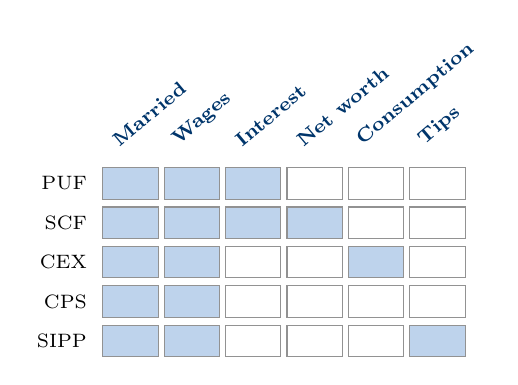
\begin{tikzpicture}[x=0.78cm, y=0.5cm]
        % columns: married, wages, interest, net worth, consumption, tips
        \foreach \lab [count=\j] in {Married, Wages, Interest, Net worth, Consumption, Tips}
          \node[font=\scriptsize\bfseries, text=yaleblue, anchor=south west, rotate=40] at (\j-0.2,0.05) {\lab};
        % one row per source: name, then 1 = observed, 0 = not in that source
        \foreach \src/\cells [count=\i] in {PUF/{1,1,1,0,0,0}, SCF/{1,1,1,1,0,0}, CEX/{1,1,0,0,1,0},
                                            CPS/{1,1,0,0,0,0}, SIPP/{1,1,0,0,0,1}} {
          \node[font=\scriptsize, anchor=east] at (0.45,-\i+0.5) {\src};
          \foreach \c [count=\j] in \cells {
            \ifnum\c=1 \def\fc{yalemid!30}\else\def\fc{white}\fi
            \draw[yalegrey!60, fill=\fc] (\j-0.45,-\i+0.1) rectangle (\j+0.45,-\i+0.9);
          }
        }
      \end{tikzpicture}\\[0.3em]
      {\scriptsize Shaded: the variable is in that source.}
    \end{column}
    \begin{column}{0.48\textwidth}
      \small
      \begin{itemize}
        \item As with a language model, all records from every source go into one training data set.
        \vspace{0.3em}
        \item One neural network is trained on the whole data set. It learns the distribution of each
              variable conditional on any set of other variables.
        \vspace{0.3em}
        \item A model that gives every such conditional distribution represents the full joint
              distribution, for example:
      \end{itemize}
    \end{column}
  \end{columns}
  \vspace{0.4em}
  {\small
  \[
    f(\text{married},\, \text{wages},\, \text{net worth})
    = f(\text{married}) \times f(\text{wages} \mid \text{married})
      \times f(\text{net worth} \mid \text{married, wages})
  \]}
\end{frame}

\begin{frame}{Model structure}
  \begin{itemize}
    \item The model is a neural network, which is a set of connected logit-like functions arranged in
          layers. Each unit takes a weighted sum of its inputs and applies a simple nonlinear
          transformation. The next layer uses those outputs as its inputs.
    \vspace{0.5em}
    \item The final layer is a multinomial logit over the 84 ranges of the variable being predicted.
    \vspace{0.5em}
    \item The network is a transformer, the type used in language models. In a transformer, the
          prediction for each variable puts more weight on the other observed variables most relevant to it.
          Variables on the record play the role that words play in a language model.
    \vspace{0.5em}
    \item Our model has 4 layers and about 1.4 million parameters.
  \end{itemize}
\end{frame}

\begin{frame}{Model estimation}
  \begin{columns}[T]
    \begin{column}{0.53\textwidth}
      \footnotesize
      \begin{enumerate}
        \item Draw a record from the training data. The source and year are always observed.
        \item Hide a random subset of the record's variables.
        \item Compute the model's predicted distribution for each hidden variable, conditional on the observed ones.
        \item Compute the log probability assigned to each true value, multiplied by the record's survey weight.
        \item Adjust each parameter by a small amount in the direction that increases this sum.
      \end{enumerate}
      \vspace{0.3em}
      This is repeated over the full training data 80 times.
    \end{column}
    \begin{column}{0.44\textwidth}
      \small
      \[
        \max_{\theta}\; \sum_{i} w_i \!\!\sum_{j\ \text{hidden}}\!\! \log p_\theta\big(x_{ij} \mid \text{shown}_i\big)
      \]
      \vspace{0.2em}
      \begin{itemize}
        \footnotesize
        \item The objective is a weighted sum of conditional log likelihoods, so the estimator is similar to maximum likelihood.
        \item The parameters are estimated by gradient descent.
        \item High-income records receive additional weight.
        \item Variables missing from a source are never predicted for that source's records.
      \end{itemize}
    \end{column}
  \end{columns}
\end{frame}

\begin{frame}{Model output for one variable}
  \begin{columns}[c]
    \begin{column}{0.52\textwidth}
      \centering
      {\small Distribution of mortgage interest for married PUF filers in 2015\\
       with AGI between the 75th and 90th percentiles}\\[0.6em]
      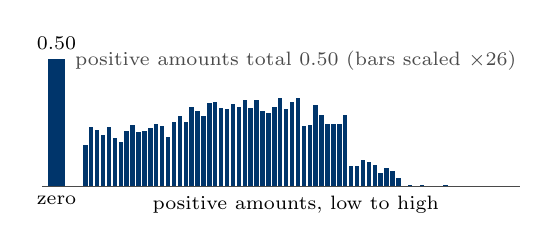
\begin{tikzpicture}[x=0.075cm, y=3.2cm]
        \fill[yaleblue] (-6,0) rectangle (-3,0.5045);
        \node[font=\scriptsize, anchor=south] at (-4.5,0.5045) {0.50};
        \foreach \k/\h in {0/0.1639, 1/0.2340, 2/0.2236, 3/0.2018, 4/0.2340, 5/0.1904, 6/0.1771, 7/0.2207, 8/0.2425, 9/0.2160, 10/0.2188, 11/0.2321, 12/0.2453, 13/0.2387, 14/0.1961, 15/0.2558, 16/0.2804, 17/0.2539, 18/0.3154, 19/0.2974, 20/0.2776, 21/0.3315, 22/0.3353, 23/0.3088, 24/0.3060, 25/0.3278, 26/0.3164, 27/0.3410, 28/0.3098, 29/0.3439, 30/0.2993, 31/0.2889, 32/0.3164, 33/0.3505, 34/0.3050, 35/0.3325, 36/0.3514, 37/0.2378, 38/0.2435, 39/0.3240, 40/0.2823, 41/0.2453, 42/0.2453, 43/0.2491, 44/0.2832, 45/0.0824, 46/0.0796, 47/0.1033, 48/0.0957, 49/0.0843, 50/0.0540, 51/0.0710, 52/0.0625, 53/0.0322, 54/0.0009, 55/0.0047, 56/0.0009, 57/0.0038, 58/0.0019, 59/0.0009, 60/0.0009, 61/0.0066, 62/0.0028, 64/0.0009, 66/0.0019, 69/0.0009}
          \fill[yaleblue] (\k,0) rectangle (\k+0.75,\h);
        \draw[yalegrey] (-7,0) -- (74,0);
        \node[font=\scriptsize, anchor=north] at (-4.5,0) {zero};
        \node[font=\scriptsize, anchor=north] at (36,0) {positive amounts, low to high};
        \node[font=\scriptsize, anchor=south, text=yalegrey] at (36,0.42) {positive amounts total 0.50 (bars scaled $\times 26$)};
      \end{tikzpicture}
    \end{column}
    \begin{column}{0.46\textwidth}
      \small
      \begin{itemize}
        \item Each dollar amount is divided into 84 ranges: zero, 10 ranges for losses
              and 73 ranges for positive amounts. The ranges are narrower at the top.
        \vspace{0.3em}
        \item The model gives a probability for each range rather than a single predicted value.
        \vspace{0.3em}
        \item The inputs are the data source, the year and any other variables known for the unit.
      \end{itemize}
    \end{column}
  \end{columns}
  \slidenote{Probabilities are shares of records in the latest run's generated sample.}
\end{frame}

% Two-panel slides: the sentence (new) and the record (from variant A).
% Horizontal probability bars at the origin: #1 a list of label/probability/drawn (1 = the drawn value).
\newcommand{\hbars}[1]{%
  \foreach \lab/\p/\d [count=\i] in {#1} {
    \ifnum\d=1 \def\bc{yaleblue}\def\tf{\bfseries}\else\def\bc{yalemid!35}\def\tf{}\fi
    \node[anchor=east, font=\scriptsize\tf] at (-0.05,-\i*0.42) {\lab};
    \fill[\bc] (0,-\i*0.42-0.14) rectangle ++(\p*5.5,0.28);
    \node[anchor=west, font=\scriptsize\tf] at (\p*5.5+0.05,-\i*0.42) {\p};
  }}
% One row of the record being written: #1 row number, #2 item, #3 value, #4 the slide it is drawn on
\newcommand{\recrow}[4]{%
  \onslide<#4->{
    \node[anchor=east, font=\scriptsize, text=yalegrey] at (2.0,-#1*0.32) {#2};
    \node[anchor=west, font=\scriptsize, inner sep=1.5pt, rounded corners=1pt,
          fill=yalelight!0] at (2.1,-#1*0.32) {#3};
    \only<#4>{\node[anchor=west, font=\scriptsize, inner sep=1.5pt, rounded corners=1pt,
          fill=yalelight!45] at (2.1,-#1*0.32) {#3};}
  }}

% The same two panels for a sentence: a language model writing one word at a time.
\begin{frame}{Sentence generation in a language model}
  \begin{tikzpicture}
    \useasboundingbox (-0.2,0.6) rectangle (14.3,-5.0);
    % the sentence so far
    \node[anchor=west, font=\small\bfseries, text=yaleblue] at (0,0.3) {Sentence so far};
    \recrow{1}{word 1}{`The'}{1}
    \recrow{2}{word 2}{`school'}{2}
    \recrow{3}{word 3}{`in'}{3}
    \recrow{4}{word 4}{`New'}{4}
    \recrow{5}{word 5}{`Haven'}{5}
    \recrow{6}{word 6}{`is'}{6}
    \recrow{7}{word 7}{`Yale'}{7}
    \draw[yalelightgrey] (4.9,0.4) -- (4.9,-4.8);

    % what the model returns at this step
    \begin{scope}[shift={(6.6,0)}]
      \only<1>{
        \node[anchor=north west, text width=7.3cm, font=\small] at (-1.3,0.4)
          {The sentence begins with `The'.\\[0.6em]
           The model then gives a probability for each possible next word.};
      }
      \only<2>{
        \node[anchor=west, font=\small\bfseries, text=yaleblue] at (-1.3,0.3) {Next word?};
        \begin{scope}[shift={(0,-0.3)}]\hbars{`first'/0.05/0, `new'/0.03/0, `school'/0.02/1, `city'/0.02/0, \textit{other}/0.88/0}\end{scope}
      }
      \only<3>{
        \node[anchor=west, font=\small\bfseries, text=yaleblue] at (-1.3,0.3) {Next word?};
        \begin{scope}[shift={(0,-0.3)}]\hbars{`is'/0.18/0, `district'/0.15/0, `board'/0.10/0, `in'/0.08/1, `year'/0.06/0, \textit{other}/0.43/0}\end{scope}
      }
      \only<4>{
        \node[anchor=west, font=\small\bfseries, text=yaleblue] at (-1.3,0.3) {Next word?};
        \begin{scope}[shift={(0,-0.3)}]\hbars{`the'/0.30/0, `question'/0.12/0, `New'/0.05/1, `my'/0.04/0, \textit{other}/0.49/0}\end{scope}
      }
      \only<5>{
        \node[anchor=west, font=\small\bfseries, text=yaleblue] at (-1.3,0.3) {Next word?};
        \begin{scope}[shift={(0,-0.3)}]\hbars{`York'/0.62/0, `Jersey'/0.09/0, `Haven'/0.08/1, `Orleans'/0.04/0, \textit{other}/0.17/0}\end{scope}
        \node[anchor=north west, text width=7.3cm, font=\small] at (-1.3,-2.9)
          {The drawn word is not always the most likely one.};
      }
      \only<6>{
        \node[anchor=west, font=\small\bfseries, text=yaleblue] at (-1.3,0.3) {Next word?};
        \begin{scope}[shift={(0,-0.3)}]\hbars{`is'/0.22/1, `was'/0.12/0, `has'/0.09/0, `area'/0.05/0, \textit{other}/0.52/0}\end{scope}
      }
      \only<7>{
        \node[anchor=west, font=\small\bfseries, text=yaleblue] at (-1.3,0.3) {Next word?};
        \begin{scope}[shift={(0,-0.3)}]\hbars{`a'/0.20/0, `Yale'/0.18/1, `the'/0.08/0, `closed'/0.05/0, \textit{other}/0.49/0}\end{scope}
        \node[anchor=north west, text width=7.3cm, font=\small] at (-1.3,-2.9)
          {Each word is drawn conditional on all previous words. Records are generated in the same way.};
      }
    \end{scope}
  \end{tikzpicture}
  \slidenote{Made-up probabilities.}
\end{frame}

\begin{frame}{Record generation}
  \begin{tikzpicture}
    \useasboundingbox (-0.2,0.6) rectangle (14.3,-5.0);
    % the record so far
    \node[anchor=west, font=\small\bfseries, text=yaleblue] at (0,0.3) {Record so far};
    \recrow{1}{source}{PUF}{1}
    \recrow{2}{year}{2015}{1}
    \recrow{3}{filer}{yes}{1}
    \recrow{4}{AGI group}{75th--90th percentile}{1}
    \recrow{5}{married}{yes}{2}
    \recrow{6}{dependents}{2}{3}
    \recrow{7}{age range}{35--44}{4}
    \recrow{8}{filing status}{joint}{5}
    \recrow{9}{child credit kids}{2}{5}
    \recrow{10}{wages}{82nd--84th pct.\ band}{6}
    \recrow{11}{mortgage int.}{66th--68th pct.\ band}{7}
    \recrow{12}{dividends}{40th--42nd pct.\ band}{8}
    \recrow{13}{Schedule C}{zero}{8}
    \recrow{14}{\dots}{about 90 tax items}{8}
    \draw[yalelightgrey] (4.9,0.4) -- (4.9,-4.8);

    % what the model returns at this step
    \begin{scope}[shift={(6.6,0)}]
      \only<1>{
        \node[anchor=north west, text width=7.3cm, font=\small] at (-1.3,0.4)
          {The source, year, filer status and AGI group are fixed before any draws.\\[0.6em]
           The model then gives a probability for each value of the next variable.};
      }
      \only<2>{
        \node[anchor=west, font=\small\bfseries, text=yaleblue] at (-1.3,0.3) {Next variable: married};
        \begin{scope}[shift={(0,-0.3)}]\hbars{no/0.29/0, yes/0.71/1}\end{scope}
      }
      \only<3>{
        \node[anchor=west, font=\small\bfseries, text=yaleblue] at (-1.3,0.3) {Next variable: dependents};
        \begin{scope}[shift={(0,-0.3)}]\hbars{0/0.49/0, 1/0.19/0, 2/0.20/1, 3+/0.13/0}\end{scope}
      }
      \only<4>{
        \node[anchor=west, font=\small\bfseries, text=yaleblue] at (-1.3,0.3) {Next variable: age range};
        \begin{scope}[shift={(0,-0.3)}]\hbars{under 26/0.00/0, 26--34/0.16/0, 35--44/0.42/1, 45--54/0.33/0, 55--64/0.08/0, 65+/0.01/0}\end{scope}
      }
      \only<5>{
        \node[anchor=north west, text width=7.3cm, font=\small] at (-1.3,0.4)
          {Filing status and the number of child tax credit children are drawn in the same way.};
      }
      \only<6>{
        \node[anchor=west, font=\small\bfseries, text=yaleblue] at (-1.3,0.3) {Next variable: wages};
        % zero band, then the 73 positive bands (bands, not dollars, on the axis)
        \fill[yalemid!35] (-1.0,-2.6) rectangle ++(0.1,0.1206);
        \foreach \b/\hgt in {1/0.0302, 2/0.0060, 6/0.0121, 8/0.0121, 13/0.0060, 18/0.0181, 19/0.0060, 20/0.0241, 21/0.0060, 22/0.0181, 23/0.0121, 24/0.0362, 25/0.0060, 26/0.0121, 27/0.0181, 28/0.0483, 29/0.0483, 30/0.0241, 31/0.0302, 32/0.0483, 33/0.0663, 34/0.0603, 35/0.1025, 36/0.1508, 37/0.1810, 38/0.2594, 39/0.4403, 40/1.3029, 41/1.4838, 42/1.8457, 43/1.6587, 44/1.9000, 45/1.8216, 46/1.0254, 47/0.8143, 48/0.0784, 49/0.0241, 50/0.0181, 51/0.0302, 53/0.0060, 54/0.0060, 59/0.0060} {
          \ifnum\b=42 \def\bc{yaleblue}\else\def\bc{yalemid!35}\fi
          \fill[\bc] (-0.75+\b*0.08,-2.6) rectangle ++(0.06,\hgt);
        }
        \draw[yalegrey] (-1.1,-2.6) -- (5.2,-2.6);
        \foreach \x/\lab in {-0.95/zero, 1.33/p50, 2.93/p90, 3.65/p99, 4.37/p99.9} {
          \draw[yalegrey] (\x,-2.6) -- ++(0,-0.08);
          \node[font=\tiny, anchor=north] at (\x,-2.66) {\lab};
        }
        \node[anchor=north west, text width=7.3cm, font=\small] at (-1.3,-3.2)
          {The drawn value (dark) is the band from the 82nd to the 84th percentile of wage earners.};
      }
      \only<7>{
        \node[anchor=west, font=\small\bfseries, text=yaleblue] at (-1.3,0.3) {Next variable: mortgage interest};
        % a tall bar for zero, then the positive bands (not to scale with the zero bar)
        \fill[yalemid!35] (-1.0,-2.6) rectangle ++(0.1,1.9);
        \node[font=\scriptsize, anchor=south] at (-0.95,-0.7) {0.46};
        \foreach \b/\hgt in {1/0.0250, 2/0.0750, 3/0.1000, 4/0.0500, 5/0.0250, 6/0.1500, 7/0.0500, 8/0.2000, 9/0.3000, 10/0.0750, 11/0.2750, 12/0.3000, 13/0.3750, 14/0.2000, 15/0.2750, 16/0.3250, 17/0.3250, 18/0.1750, 19/0.4000, 20/0.5750, 21/0.5500, 22/0.2500, 23/0.5750, 24/0.6000, 25/0.4250, 26/0.4750, 27/0.6250, 28/0.5250, 29/0.7250, 30/0.5500, 31/0.6750, 32/0.6750, 33/0.6250, 34/0.9000, 35/0.6250, 36/0.6250, 37/0.5500, 38/0.3750, 39/0.4250, 40/0.4250, 41/0.4250, 42/0.1250, 43/0.1500, 44/0.4750, 45/0.4250, 46/0.0750, 47/0.1000, 48/0.1250, 49/0.3000, 50/0.2500, 51/0.0500, 52/0.0750, 53/0.1000, 54/0.0500, 62/0.0250} {
          \ifnum\b=34 \def\bc{yaleblue}\else\def\bc{yalemid!35}\fi
          \fill[\bc] (-0.75+\b*0.08,-2.6) rectangle ++(0.06,\hgt);
        }
        \node[font=\scriptsize, anchor=south] at (1.65,-1.2) {positive amounts total 0.54 (not to scale)};
        \draw[yalegrey] (-1.1,-2.6) -- (5.2,-2.6);
        \foreach \x/\lab in {-0.95/zero, 1.33/p50, 2.93/p90, 3.65/p99, 4.37/p99.9} {
          \draw[yalegrey] (\x,-2.6) -- ++(0,-0.08);
          \node[font=\tiny, anchor=north] at (\x,-2.66) {\lab};
        }
        \node[anchor=north west, text width=7.3cm, font=\small] at (-1.3,-3.2)
          {The drawn value (dark) is the band from the 66th to the 68th percentile of filers with mortgage interest.};
      }
      \only<8>{
        \node[anchor=north west, text width=7.3cm, font=\small] at (-1.3,0.4)
          {The remaining tax variables are drawn in the same way, in a random order. Totals such as AGI are computed as sums of the drawn components.\\[0.5em]
           Survey variables are drawn next: the balance sheet from the SCF and consumption from the CEX.\\[0.5em]
           Each range is converted to dollars by drawing a real amount from that range and growing it to the target year.};
      }
    \end{scope}
  \end{tikzpicture}
  \slidenote{Probabilities are shares of records in the latest run's generated sample that match the record so far.}
\end{frame}

\begin{frame}{The generated sample}
  \begin{itemize}
    \item 400,000 filer records are drawn as the PUF would record them, with a fixed number in each of 12 AGI groups.
    \vspace{0.4em}
    \item Each record's starting weight is the number of returns in its AGI group divided by the number of records drawn in that group.
    \vspace{0.4em}
    \item 54,379 non-filer records are drawn as the CPS would record them.
    \vspace{0.4em}
    \item Each record also receives survey variables: the balance sheet from the SCF, consumption from the CEX and tips from the SIPP.
    \vspace{0.4em}
    \item Each record is a new draw from the joint distribution rather than a copy of a survey household.
  \end{itemize}
  \slidenote{Latest run, 2019 file.}
\end{frame}

\begin{frame}{Post-training: reweighting to targets}
  \small
  Records are kept as drawn. New weights $w_i$ are chosen to stay as close as possible to the starting weights $w^0_i$:
  \[
    \min_{w}\; \sum_i w_i \log\frac{w_i}{w^0_i}
    \quad\text{such that every target is within } \pm 1 \text{ standard error (SCF: } \tfrac12\text{)}
  \]
  \vspace{-0.6em}
  \begin{itemize}
    \item This is the same distance measure used in raking.
    \item For 2019 there are 753 targets, all of which are met. They include IRS tables by AGI, filing status and age,
          business income, W-2 tips, non-filer counts, SCF wealth and CEX spending.
  \end{itemize}
\end{frame}

% Source: tilt/seed20261016/file_2019.parquet, weight over weight_start, 454,379 records (27 October run).
% Effective sample: (sum w)^2 / sum w^2, as solver.py; 87.2% matches summary.md.
\begin{frame}{Distance of weight movement}
  \begin{columns}[T]
    \begin{column}{0.48\textwidth}
      \centering
      \small
      \begin{tabular}{@{}lrr@{}}
        \toprule
        Ratio of new to starting & \multicolumn{2}{c}{Share of} \\
        weight within a factor of & records & returns \\
        \midrule
        1.05 & 15\% & 20\% \\
        1.1  & 26\% & 36\% \\
        1.25 & 44\% & 61\% \\
        1.5  & 58\% & 77\% \\
        2    & 70\% & 86\% \\
        4    & 81\% & 92\% \\
        10   & 96\% & 99\% \\
        \bottomrule
      \end{tabular}
    \end{column}
    \begin{column}{0.48\textwidth}
      \small
      \begin{itemize}
        \item A factor of 2 means the new weight is between half and double the starting weight.
        \vspace{0.4em}
        \item The effective sample size is $(\sum w)^2 / \sum w^2$. It equals the number of records
              when all weights are equal and declines as the weights become more unequal.
        \vspace{0.4em}
        \item Reweighting retains 87 percent of the effective sample size, which falls from
              280,800 to 244,700 (out of 454,379 records).
      \end{itemize}
    \end{column}
  \end{columns}
  \slidenote{Latest run, 2019 file. Share of returns is measured with starting weights.}
\end{frame}

% ===========================================================================
% 5. Challenges. Interest numbers: 2016 SCF (tax year 2015) against the 2015 PUF,
% weighted, married with wages $75k-200k (21 October deck; source report in
% rebuild/explore/2026-10-21/reporting_formula/, as cited there).
% ===========================================================================

\begin{frame}{Challenge: measurement differences between surveys and tax returns}
  \centering
  \begin{tikzpicture}
    \begin{axis}[ybar, width=12cm, height=5.4cm, bar width=14pt, ymin=0, ymax=32,
        symbolic x coords={\$1--100, \$100--500, \$500--2k, \$2k--10k, \$10k+},
        xtick=data, xticklabel style={font=\small}, yticklabel style={font=\small},
        ylabel={Per 100 tax units}, ylabel style={font=\small},
        xlabel={Interest received in the year}, xlabel style={font=\small},
        legend style={font=\small, draw=none, at={(0.97,0.95)}, anchor=north east},
        axis x line*=bottom, axis y line*=left, enlarge x limits=0.12,
        nodes near coords, every node near coord/.append style={font=\scriptsize}]
      \addplot[fill=yaleblue, draw=none] coordinates
        {(\$1--100,28) (\$100--500,13) (\$500--2k,4) (\$2k--10k,2) (\$10k+,1)};
      \addplot[fill=yalelight!70, draw=none] coordinates
        {(\$1--100,8) (\$100--500,6) (\$500--2k,3) (\$2k--10k,3) (\$10k+,1)};
      \legend{PUF: reported on return (48 total), SCF: reported in survey (21 total)}
    \end{axis}
  \end{tikzpicture}

  \vspace{0.3em}
  The gap is concentrated in small amounts, which often go unreported in the survey. Above \$2,000 the two sources agree.
  \slidenote{Married, wages \$75--200k. 2015 PUF and 2016 SCF (tax year 2015), weighted.}
\end{frame}

\begin{frame}{The fix: assigning values for false negatives}
  \centering
      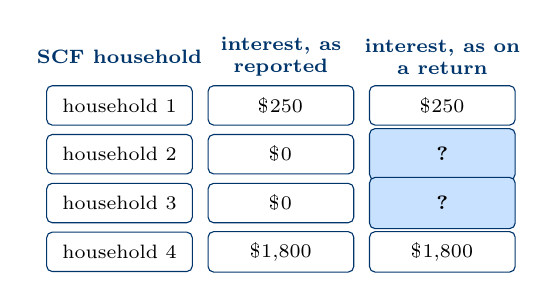
\begin{tikzpicture}[x=2.05cm, y=0.62cm,
          c/.style={tok, minimum width=1.85cm, minimum height=0.5cm, font=\scriptsize}]
        \node[font=\scriptsize\bfseries, text=yaleblue] at (1,0) {SCF household};
        \node[font=\scriptsize\bfseries, text=yaleblue, align=center] at (2,0) {interest, as\\reported};
        \node[font=\scriptsize\bfseries, text=yaleblue, align=center] at (3,0) {interest, as on\\a return};
        \foreach \r/\said/\ret/\hd in {1/\$250/\$250/0, 2/\$0/?/1, 3/\$0/?/1, 4/{\$1,800}/{\$1,800}/0} {
          \node[c] at (1,-\r) {household \r};
          \node[c] at (2,-\r) {\said};
          \ifnum\hd=1 \node[c, blank, font=\scriptsize\bfseries] at (3,-\r) {\ret}; \else \node[c] at (3,-\r) {\ret}; \fi
        }
      \end{tikzpicture}

  \vspace{0.4em}
  \raggedright
  \small
  \begin{itemize}
    \item Each SCF household has two versions of interest, dividends and capital gains.
    \item The first version is the survey answer, which is never changed.
    \item The second version is the amount that would appear on a tax return.
          Households that report an amount keep it. Households that report zero may be assigned a value.
    \item PUF records have only the tax-return version, so both sources use the same definition.
  \end{itemize}
\end{frame}

% Fill-in mechanics: research/rebuild/FEATURES.md, "Function 2: two slots, filled during training".
\begin{frame}{Assigning values for false negatives during pretraining}
  \begin{columns}[T]
    \begin{column}{0.44\textwidth}
      \centering
      \small
      \begin{tabular}{lrrr}
        \toprule
        Per 100 couples & PUF & SCF & Fill in \\
        \midrule
        \$1--100      & 28 & 8 & 20 \\
        \$100--500    & 13 & 6 & 7 \\
        \$500--2k     & 4  & 3 & 2 \\
        \$2k and over & 3  & 3 & 0 \\
        \midrule
        Any           & 48 & 21 & 28 \\
        \bottomrule
      \end{tabular}

      \vspace{0.8em}
      \raggedright
      The PUF determines the number and size of fill-ins.
      The rest of the SCF record determines the households that receive them.
    \end{column}
    \begin{column}{0.53\textwidth}
      \footnotesize
      \begin{enumerate}
        \item At the start of each pass through the data (from the third), the model computes each
              zero-reporting household's probability of holding an amount in each range.
        \item This probability is the model's probability that the household reports that range,
              given the rest of its record, times (PUF share $\div$ SCF share $-$ 1) for its type
              (married, dependents, wage band), divided by its probability of reporting zero.
        \item Each batch of records draws new fill-ins from these probabilities. The model is
              trained on the tax-return version of the variable.
        \item The probabilities use only the reported values and the PUF, never earlier fill-ins.
      \end{enumerate}
    \end{column}
  \end{columns}
  \slidenote{Table: married, wages \$75--200k; 2015 PUF and 2016 SCF, weighted. Probabilities are capped at 100 percent.}
\end{frame}

% Grouped weighting: research/rebuild/FEATURES.md, "Weights: grouped weighting" and generation.
\begin{frame}{Challenge: sample weights}
  \begin{columns}[T]
    \begin{column}{0.48\textwidth}
      \textbf{\color{yaleblue}Problem}\\[0.4em]
      \small
      \begin{tabular}{@{}lr@{}}
        \toprule
        PUF record & Returns it stands for \\
        \midrule
        AGI below the median & about 1,390 \\
        AGI at p99.99 and up & about 1.6 \\
        \bottomrule
      \end{tabular}

      \vspace{0.8em}
      With survey weights, the model sees very little of the top, which is 0.02 percent of returns.
      With equal weights, the model learns the sample rather than the population.
    \end{column}
    \begin{column}{0.48\textwidth}
      \textbf{\color{yaleblue}Approach: grouped weighting}\\[0.4em]
      \footnotesize
      \begin{enumerate}
        \item Records are divided into groups: 12 AGI groups in the PUF and 5 income classes in the SCF.
        \item In estimation, each record is weighted by its survey weight times $q$, where $q$ is the
              number of records divided by the total survey weight in its group.
        \item Within a group, records are weighted by survey weight. Across groups, they are weighted by
              record count. The top AGI group rises from 0.02 to 4.6 percent of the PUF's estimation weight.
        \item In generation, a fixed number of records is drawn in each group and weighted by $1/q$,
              which reverses the adjustment exactly.
      \end{enumerate}
    \end{column}
  \end{columns}
\end{frame}

\begin{frame}{Other challenges}
  \begin{itemize}
    \item \textbf{Tax unit construction.} Surveys record households. Each household is divided into
          tax units using a common set of rules. A filing model then determines whether each unit files.
    \vspace{0.5em}
    \item \textbf{Changes in tax law.} TCJA reduced the number of itemizers. New items such as the
          tips and overtime deductions do not appear on any past return.
    \vspace{0.5em}
    \item \textbf{The top of the distribution.} Every source has few very high-income records.
    \vspace{0.5em}
    \item \textbf{Future years.} There is no microdata for future years, only a small number of projected totals.
    \vspace{0.5em}
    \item \textbf{Validation.} No source contains every variable, so some relationships cannot be
          checked against data.
  \end{itemize}
\end{frame}

% ===========================================================================
% 6. Where we are
% ===========================================================================

\begin{frame}{Status}
  \begin{itemize}
    \item A 2019 file with 400,000 filer records and 54,379 non-filer records
    \vspace{0.4em}
    \item Five sources: the 2015 PUF, SCF, CEX, CPS and SIPP. Each survey is divided into tax units
          using the same rules.
    \vspace{0.4em}
    \item All PUF variables, plus a balance sheet, consumption, tips and auto loan interest
    \vspace{0.4em}
    \item 753 targets, all met within their standard errors, including IRS tables by AGI, filing
          status and age, the top 1, 0.1 and 0.01 percent, W-2 tips and SCF wealth
  \end{itemize}
\end{frame}

\begin{frame}{Next steps}
  \begin{itemize}
    \item Rule-based variables added after generation: credit eligibility, mortality probabilities,
          unrealized gains and capital gains basis
    \vspace{0.4em}
    \item Output files in Tax-Simulator's input format, followed by a first Tax-Simulator run
    \vspace{0.4em}
    \item A tax calculator within post-training, to allow targets on computed tax
    \vspace{0.4em}
    \item Other years: 2015 to 2023, followed by the projection years
    \vspace{0.4em}
    \item The top of the distribution: the PUF's aggregate records and the Forbes 400
  \end{itemize}
\end{frame}

\begin{frame}[plain,noframenumbering,c]
  \begin{center}
    {\color{yaleblue}\Large\bfseries Questions}
  \end{center}
\end{frame}

% ---------------------------------------------------------------------------
% Parked: the 24 October intro slides, kept in case any are wanted back.
% ---------------------------------------------------------------------------
\iffalse

\begin{frame}{What do we need?}
  % Click 1: the need as one sentence. Click 2: its words down the side, each explained.
  \only<1>{%
    \vfill
    \begin{center}
      {\LARGE\bfseries\color{yaleblue} Realistic synthetic augmented tax unit microdata}
    \end{center}
    \vfill
  }
  \only<2>{%
  \vspace{0.6em}
  \renewcommand{\arraystretch}{1.4}
  \begin{tabular}{@{}r@{\hspace{1.2em}}>{\raggedright\arraybackslash}p{0.74\textwidth}@{}}
    {\large\bfseries\color{yaleblue} Realistic}   & joint distributions across all variables are respected; aggregate targets are hit \\
    {\large\bfseries\color{yaleblue} Synthetic}   & files for historical and future years \\
    {\large\bfseries\color{yaleblue} Augmented}   & variables not on tax returns, and people who don't file \\
    {\large\bfseries\color{yaleblue} Tax unit}    & the unit that files or would file: non-filers included, households split \\
    {\large\bfseries\color{yaleblue} Microdata}   & individual records, so we can calculate taxes in detail \\
  \end{tabular}
  }
\end{frame}

% What each source has, and which years. Simplified: shading marks whether a
% source carries the item at all, not how well. Tax years.
\begin{frame}{What do we have?}
  \centering
  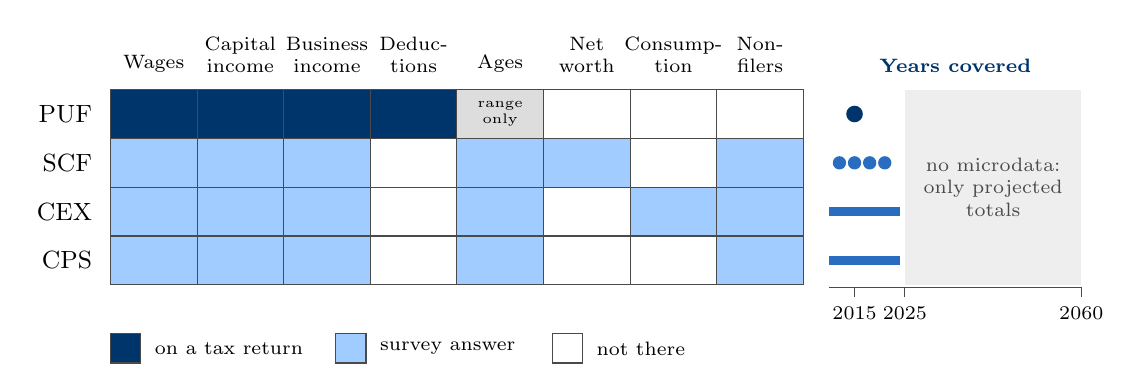
\begin{tikzpicture}[x=1.1cm, y=0.62cm]
    % column labels
    \foreach \lab [count=\i] in {Wages, {Capital\\income}, {Business\\income}, {Deduc-\\tions},
        Ages, {Net\\worth}, {Consump-\\tion}, {Non-\\filers}} {
      \node[font=\scriptsize, align=center, anchor=south] at (\i-0.5, 0.15) {\lab};
    }
    % rows: F = on a tax return, P = survey answer, N = not there
    \foreach \lab/\codes [count=\j] in {
        PUF/{cF,cF,cF,cF,cN,cN,cN,cN},
        SCF/{cP,cP,cP,cN,cP,cP,cN,cP},
        CEX/{cP,cP,cP,cN,cP,cN,cP,cP},
        CPS/{cP,cP,cP,cN,cP,cN,cN,cP}} {
      \node[font=\small, anchor=east] at (-0.1, -\j+0.5) {\lab};
      \foreach \c [count=\i] in \codes {
        \draw[\c, draw=yalegrey] (\i-1, -\j) rectangle (\i, -\j+1);
      }
    }
    % the PUF has the primary filer's age range only, and for most records
    \fill[yalelightgrey] (4,-1) rectangle (5,0);
    \draw[yalegrey] (4,-1) rectangle (5,0);
    \node[font=\tiny, align=center] at (4.5,-0.5) {range\\only};
    % legend
    \begin{scope}[shift={(0,-5.6)}]
      \draw[cF, draw=yalegrey] (0,0) rectangle (0.35,0.6);
      \node[font=\scriptsize, anchor=west] at (0.4,0.3) {on a tax return};
      \draw[cP, draw=yalegrey] (2.6,0) rectangle (2.95,0.6);
      \node[font=\scriptsize, anchor=west] at (3.0,0.3) {survey answer};
      \draw[cN, draw=yalegrey] (5.1,0) rectangle (5.45,0.6);
      \node[font=\scriptsize, anchor=west] at (5.5,0.3) {not there};
    \end{scope}

    % Click 2: which years each source covers, on a line from 2010 to 2060
    \onslide<2>{
    \begin{scope}[shift={(8.3,0)}, x=0.064cm]
      \node[font=\scriptsize\bfseries, text=yaleblue, anchor=south] at (25,0.15) {Years covered};
      % no microdata after the last survey year
      \fill[yalelightgrey!50] (15,-4.0) rectangle (50,0);
      \node[font=\scriptsize, align=center, text=yalegrey] at (32.5,-2) {no microdata:\\only projected\\totals};
      % PUF: 2015 only
      \fill[yaleblue] (5,-0.5) circle (3pt);
      % SCF: every third tax year
      \foreach \yr in {2012,2015,2018,2021} \fill[yalemid] (\yr-2010,-1.5) circle (2.4pt);
      % CEX and CPS: every year
      \draw[yalemid, line width=3pt] (0,-2.5) -- (14,-2.5);
      \draw[yalemid, line width=3pt] (0,-3.5) -- (14,-3.5);
      % axis under the last row
      \draw[yalegrey] (0,-4.05) -- (50,-4.05);
      \foreach \yr in {2015, 2025, 2060} {
        \draw[yalegrey] (\yr-2010,-4.05) -- (\yr-2010,-4.25);
        \node[font=\scriptsize, anchor=north] at (\yr-2010,-4.25) {\yr};
      }
    \end{scope}
    }
  \end{tikzpicture}

  \vspace{0.6em}
  No source has everything, and only one year has tax returns.
  \slidenote{Simplified. Years are tax years.}
\end{frame}

\begin{frame}{Why can't we just combine them?}
  \begin{itemize}
    \item \textbf{Different units.} Surveys count households; returns count tax units.
          One household can hold several returns, and some people file none.
    \vspace{0.6em}
    \item \textbf{Different definitions.} A return caps capital losses at \$3,000;
          survey wages are counted before pre-tax deductions.
    \vspace{0.6em}
    \item \textbf{Different measurement.} Small amounts go unreported: of every 100 couples,
          48 show interest on their returns, but only 21 tell the SCF they have any.
  \end{itemize}
  \slidenote{Interest: married couples with wages of \$75--200k, 2015 PUF and 2016 SCF (tax year 2015), weighted.}
\end{frame}

\begin{frame}{The task}
  \centering
  \vspace{1.5em}
  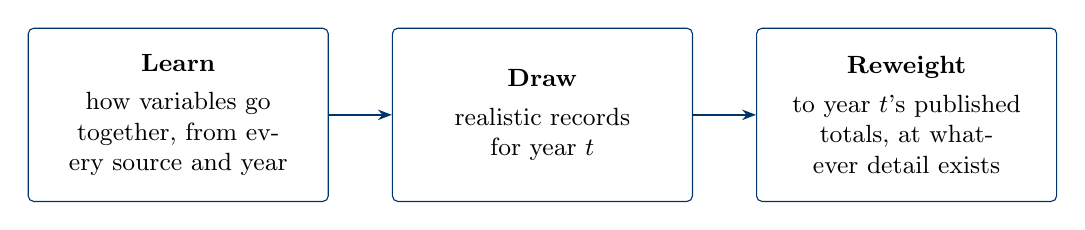
\begin{tikzpicture}
    \node[box, text width=3.6cm, minimum height=2.2cm, font=\small] (learn)
      {\textbf{Learn}\\[3pt] how variables go together, from every source and year};
    \node[box, text width=3.6cm, minimum height=2.2cm, font=\small, right=0.8cm of learn] (draw)
      {\textbf{Draw}\\[3pt] realistic records for year $t$};
    \node[box, text width=3.6cm, minimum height=2.2cm, font=\small, right=0.8cm of draw] (hit)
      {\textbf{Reweight}\\[3pt] to year $t$'s published totals, at whatever detail exists};
    \draw[arr] (learn) -- (draw);
    \draw[arr] (draw) -- (hit);
  \end{tikzpicture}
\end{frame}

\fi

\end{document}
